\documentclass[../mit-general-chemistry.tex]{subfiles}
\begin{document}


\chapter{Acid-base equilibrium}




There are three main theories definitions on acids and
bases. Arrhenius gives a narrow definition of acids and bases. An {\em
  acid} is a substance that produce hydrogen ions, protons (\ce{H+})
when solved in water. A base is a substance that increase the
hydroxide (\ce{OH-}) concentration.


In Brønstedt-Lowry's definition, an acid is a substance that can {\em
  donate a proton} (hydrogen ion). A base is a substance that can {\em accept a
  proton}.

\paragraphbreak
  
If we look at the reaction where acetic acid is dissolved in water
forming acetate ion and oxonium (hydonium) ion.

\ceeqstar{
  $\underset{\color{red}\text{acid}~\rightarrow}{\ce{CH3COOH(aq)}}$
  +
  $\underset{\color{red}\text{base}~\rightarrow}{\ce{H2O(l)}}$
  <=>
  $\underset{\color{red}\leftarrow~\text{acid}}{\ce{H3O^+(aq)}}$
  +
  $\underset{\color{red}\leftarrow~\text{base}}{\ce{CH3COO^-(aq)}}$
}

Acetic acid (\ce{CH3COOH}) acts as an acid when it is solved in water
(the reaction, going to the right). It donates a proton to water. In
this reaction, water acts as a base, accepting a proton, forming an
oxonium (hydonium) ion.

In the reverse reaction, the roles are switched, in a sense. Now the
oxonium ion acts as an acid as it donates a proton (``back'') to the
acetate ion which acts as a base.

The {\em conjugate base} of an acid is the base that is formed when
the acid donates a proton. Conversely, a {\em conjugate acid} us the
acid that is formed as a base accepts a proton.

In the example, acetate ion is the conjugate base of acetic acid and
acetic acid is the conjugate acid of the acetate ion. The same goes
for water and the oxonium ion.

Acetic acid and acetate form a (Brønstedt) acid-base pair.


\paragraphbreak

Looking at bicarbonate anion dissolving in water into carbonate and
oxonium ions.

\ceeqstar{HCO3^-(aq) + H2O(l) <=> H3O+(aq) + CO3^2-(aq)}

This is another example of water and an acid forming
conjugate acid, base pairs.

\begin{center}
  \begin{tabular}{ll}
    Acid & Base \\
    \midrule
    \ce{HCO3^-} & \ce{CO3^2-} \\
    \ce{H3O+} & \ce{H2O} \\
  \end{tabular}
\end{center}

Bicarbonate can also act as a base. The same reactants, bicarbonate
and water, can also form carbonic acid and hydroxide.

\ceeqstar{HCO3^-(aq) + H2O <=> H2CO3 + OH-}

Here, water acts as an acid with the conjugate base hydroxide.

\begin{center}
  \begin{tabular}{ll}
    Acid & Base \\
    \midrule
    \ce{H2CO3} & \ce{HCO3^-} \\
    \ce{H2O} & \ce{OH-} \\
  \end{tabular}
\end{center}



A substance that can act as either a base or an acid is said to be
{\em amphoteric}. To figure out wether an amphoteric substance is
acting like am acid or a base in a reaction we need to look at the
products for that reaction.



\paragraphbreak

A {\em Lewis base} is a chemical species that donates lone pair
electrons. A {\em Lewis acid} is a chemical species that accepts such
electrons. In other words, a Lewis acid is an electron-pair
acceptor. A Lewis base is any substance, such as the OH- ion, that can
donate a pair of non-bonding electrons. A Lewis base is therefore an
electron-pair donor.

A Lewis acid is an electron-pair acceptor, and a Lewis base is an
electron-pair donor. Another way of saying this is that a Lewis acid
has an empty atomic orbital that it can use to accept (share) an
electron pair from a mol- ecule that has a lone pair of electrons
(Lewis base).\autocite[663]{miessler2014}

The Lewis model encompasses the Brønsted–Lowry model, but the reverse
is not true.

See for instance the reaction
\begin{center}
  \schemestart
  \chemfig{H^+}
  \+
  \chemfig{\lewis{4:,N}(-[:0]H)(-[:90]H)(-[:270]H)}
  \arrow
  $\chemleft[
    \chemfig{N(-[:0]H)(-[:90]H)(-[:270]H)(-[:180]H)}
    \chemright]^+$
  \schemestop
\end{center}
where the proton acts as a Lewis acid ``accepting'' the lone pair
electrons from the nitrogen atom of the ammonia molecule which acts as
a Lewis base.

This is a much broader definition than the Arrhenius definition or the
Brønsted-Lowry definition. Lewis acid-base theory includes reactions
that doesn't include any hydrogen, as we see in
\begin{center}
  \schemestart
  \chemfig{B(-[:90]\lewis{0:2:4:,F})(-[:180]\lewis{2:4:6:,F})(-[:270]\lewis{4:6:0:,F})}
  \+
  \chemfig{\lewis{4:,N}(-[:0]H)(-[:90]H)(-[:270]H)}
  \arrow
  \chemfig{B(-[:90]\lewis{0:2:4:,F})(-[:180]\lewis{2:4:6:,F})(-[:270]\lewis{4:6:0:,F})-N(-[:0]H)(-[:90]H)(-[:270]H)}
  \schemestop
\end{center}
Here the electron-deficient BF3 molecule (there are only six electrons
around the boron) completes its octet by reacting with NH3, which has
a lone pair of electrons. (see Fig. 14.12.) In fact, as mentioned in
Chapter 8, the electron deficiency of boron trifluoride makes it very
reactive toward any electron-pair donor. That is, it is a strong Lewis
acid.\autocite[664]{miessler2014}

Lewis acid-base theory complements the oxidation-reduction class of
reactions in which electrons are transferred, whereas in Lewis'
acid-base theory they are shared.




\section{Autoionization of water}

Water is an {\em amphoteric} or {\em amphiprotic} substance, a
substance that can act as both a Brønsted acid and a Brønsted base. It
can act either as an acid or as a base. Water molecules can react with
each other in reactions known as water {\em autoprotolysis} (or ‘{\em
  autoionization}’).


\ceeq{\label{rxn:autoionization}
  $\underset{\color{blue}\text{acid}~\rightarrow}{\ce{H2O(l)}}$
  +
  $\underset{\color{red}\text{base}~\rightarrow}{\ce{H2O(l)}}$
  <=>
  $\underset{\color{red}\leftarrow~\text{acid}}{\ce{H3O+(aq)}}$
  +
  $\underset{\color{blue}\leftarrow~\text{base}}{\ce{OH-(aq)}}$
}


So, how common are these reactions in water? How acidic is a glass of
water? The answer is to be found in the equilibrium constant for
Reaction~\ref{rxn:autoionization} and how much product this
yields. When the reaction has reached equilibrium, the equilibrium
constant tells us the ratio between product concentration over
reactant concentration and this tells us just how much \ce{H2=} there
is in a glass of water.

So what is the equilibrium constant? We can use any of the equations
we've used in the previous chapter, but the common way to do this is
using
\begin{equation*}
  \ln K = - \frac{\gibbsO}{RT}
\end{equation*}
for $RT$, the ideal gas constant
(\SI{8.3144598(48)}{\joule\per\kelvin\per\mol}) times the temperature
and \gibbsO\ the Gibb's free energy of the reactants and products of
the reaction.

There are two ways we can calculate \gibbsO.
\begin{align*}
  &\gibbsO\ = \sum_{i = \text{products}} n_i \gibbsO_{f,i}
  - \sum_{j = \text{reactants}} n_j \gibbsO_{f,j} \\
  &\gibbsO\ = \enthalpyO - T\dS^0
\end{align*}

We pick one of these and calculate the \gibbsO\ from the standard Gibbs
free energy of formation for the reactants and products.

\begin{align*}
  \gibbsO\ &= \gibbs_f(\ce{H3O+}) + \gibbs_f(\ce{OH-}) - 2\cdot\gibbs_f(\ce{H2O}) = \\
  &= (-237.13) + (-157.24) - 2\cdot(-237.13)~\kjpm = \\
  &= 79.89~\kjpm
\end{align*}

For $\gibbsO\ = 79.89~\kjpm$, we expect $K$ to be small. We can
calculate it
\begin{equation*}
  \ln K = -\frac{\gibbsO}{RT}
  = -
  \frac{\SI{7.989d4}{\joule\per\mol}}{\SI{8.3145}{\joule\per\kelvin\per\mol}\cdot\SI{298}{\kelvin}}
  = -32.24
\end{equation*}

We can use this to calculate

\begin{equation*}
  \ln K = -32.24 \implies K = \num{9.962d-15} \approx \num{1d-14}
\end{equation*}

This very small number shows that only a very small proportion of
water molecules are ionized at the same time.

This $K$ has a special name, $K_w$, $w$ for water and
\ceeq{K_w = [H3O^+][OH^-]}

\begin{remark}
  Because the concentration of the solvent, \ce{H2O}, does not change
  significantly in a dilute solution, it does not enter the equilibrium
  expression. The solvent is very nearly pure. Pure liquids and pure
  solids are not included in equilibrium expressions.
\end{remark}


Because $K_w$ is an equilibrium constant, the product of
$\ce{[H3O^+][OH^-]}$ is always \num{1d-14} at \SI{298}{\kelvin} (room
temperature).




\section{\si{pH} function}


The \pH\ function is defined as
\ceeq{\pH\ = - \log_{10} [H3O^+]}
We have also the corresponding
\ceeq{\pOH = - \log_{10} [OH^-]}
The square brackets denote the concentration of a species.

Let us take the fact that $\ce{K_w = [H3O^+][OH^-] = \num{1d-14}}$ and
calculate
\begin{align*}
  \ce{[H3O^+][OH^-] &= \num{1d-14}}\\
  \ce{-\log_{10} ([H3O^+][OH^-]) &= \num{14}} \\
  \ce{-\log_{10} ([H3O^+]) -\log_{10}([OH^-]) &= \num{14}} \\
  \ce{-\log_{10} ([H3O^+]) -\log_{10}([OH^-]) &= \num{14}} \\
  \pH\ + \pOH &= 14 ~\text{at \SI{298}{\kelvin}.}\\
\end{align*}

\pH\ is the measure of the strength of an acid. It is also a
measure of the acidity of a solution. The sum of \pH\ and
\pOH is always going to be 14 at \SI{298}{\kelvin}. \pH\ of
pure (neutral) water is 7. The \pH\ of an acidic solution is going
to be lower than 7 and conversely will the \pH\ of a base solution
be higher than 7.

The United States' Environment protection agency (EPA) classifies
waste as {\em corrosive} if \pH\ is less than \num{3.0} or greater
than \num{12.5}.





\section{Strengts of acids and bases}



Considering
\ceeq{CH3COOH(aq) + H2O(l) <=> H3O^+(aq) + CH3COO^-(aq)}
again. We define the {\em acid ionization constant} for this reaction
\ceeq{K_a = \frac{[H3O^+][CH3COO^-]}{[CH3COOH]}}

The concentration of water is left out of the equation. It is the
solvent, it is pretty much pure and it's concentration will not change
much.

$K_a$ is an equilibrium constant. It is going to be \num{1.76d-5} at
\SI{25}{\celsius} for this reaction. This is a comparably small number
and that tells us that this acid is not going to ionize much in
solution. This is a measure of the strength of an acid.

An acid with a $K_a > 1$ is considered a {\em strong acid}. $K_a > 1$
means it is going to ionize almost completely. An acid with $K_a < 1$
is considered a {\em weak acid}. $K_a < 1$ means that the reaction
reaches equilibrium before much of the acid is ionized.

We are going to discuss two generic equations
\ceeq{HA(aq) + H2O(l) <=> H3O^+(aq) + A^-(aq)}
which is similar to the equation above, and
\ceeq{BH^+(aq) + H2O(l) <=> H3O^+(aq) + B(aq)}

Both \ce{A} and \ce{B} are considered to be Brønstedt acids as they
are donating protons during the reactions.

We also define
\begin{equation}
  \pKa = - \log_{10} K_a
\end{equation}

Notice that the higher the \pKa, the weaker the
acid.


\begin{remark}
  The discussion here is limited to the strength and dissociation of
  acids in aqueous solutions. In aqueous solutions a leveling efect
  occurs, due to the dissociation of water. This produces a {\em leveling
  effect} where the \pH\ of very strong acids like nitric acid,
  sulfuric acid and hydrochloric acid, all are estimated to have a
  $\pH\ = 0$~(e.g. \cite[172]{miessler2014}).

  In solution with other solvents, the acidity of these three (and
  other, similar acids) are distinguishable.
\end{remark}






\section{Bases in water}

We also consider bases and the strength of bases. In the reaction of
ammonia picking up a proton from water, forming ammonium cations, the
base ammonia is ionized into ammonium cation and water molecules
become hydroxide anions.

\ceeq{NH3(aq) + H2O(l) <=> NH4^+(aq) + OH^-(aq)\label{eq:ammonia-ionization}}

Here, ammonia acts as a Brønstedt base that accepts a proton from a
water molecule.

As we did with acids, we can define a {\em base ionization constant},
\Kb, and we define this in a similar way

\ceeq{
  \Kb = \frac{[NH4^-][OH^-]}{[NH3]}
}

The base ionization constant is an equilibrium constant for a reaction
involving the ionization of a base into it's conjugate acid. It is
calculated under the same provisions as the acid ionization
constant. This is why the concentration of the solvent, water, is
omitted.

If we calculate the base ionization constant for the reaction in
Equation~\ref{eq:ammonia-ionization} it is $\Kb = \num{1.8d-5}$ at
\SI{25}{\celsius}, which is a really small number and this tells us
that only a small amount of \ce{NH3} will ionize into \ce{NH4^+} and
\ce{OH^-} when dissolved in water and it makes \ce{NH3} a moderately {\em weak base}.


A strong base reacts essentially completely to give \ce{OH^-}. For
bases that dissolve and produce more of the conjugate acid and
hydroxide than there is left of the base when the ionization reaches
equilibrium, \Kb is going to be greater than one. For strong bases \Kb
is going to be considerably larger still.



If we write general equations for bases in water (as we did for acids)
they look like

\begin{align}
  \ce{B(aq) + H2O(l) &<=> BH^+(aq) + OH^-(aq)\quad\text{(base \ce{B} in water)}} \\
  \ce{A^-(aq) + H2O(l) &<=> AH(aq) + OH^-(aq)\quad\text{(base \ce{A^-} in water)}}
\end{align}

\Kb\ is still an equilibrium constant so the greater the \Kb\ for a
reaction, the stronger the base and, as for \Ka\ we have a similar
measure $\pKb = - \log_{10} \Kb$ with the corresponding properties for
bases: the weaker the base, the greater the \pKb. When
$[\ce{BH^+}][\ce{OH^-}] > [\ce{B}]$ or $[\ce{AH}][\ce{OH^-}] >
[\ce{A^-}]$, $\Kb > 1$ and $\pKb < 0$. \pKb\ is not used much. It is
commonly converted into \pKa.




\section{Conjugate acids and bases}


{\em The stronger the acid, the weaker it's conjugate base} and
conversely {\em the stronger the base, the weaker it's conjugate
  acid}.

This correlates well with the fact that \Ka\ and \Kb\ are equilibrium
constants; a strong acid will ionize completely, that is, the reaction
will go completely to the right before reaching equilibrium. At
equilibrium there will be alot of hydronium ions and the conjugate
base and hardly any amount of the acid. The same goes for strong
bases.



\subsection{Proof that strong bases have weak conjugate acids}


Consider Equation~\ref{eq:ammonia-ionization} again
\ceeqstar{NH3(aq) + H2O(l) <=> NH4^+(aq) + OH^-(aq)}

Ammonia is acting as a base, accepting a proton from water, forming
ammonium ions. Water acts as an acid, forming hydroxide ions as it
donates protons to ammonia.

The base ionization constant for the reaction is
\ceeqstar{
  K_b = \frac{[NH4^+][OH^-]}{[NH3]}
}


So, let's look at the next (inverse) reaction

\ceeqstar{ NH4^+(aq) + H2O(l) <=> H3O^+(aq) + NH3(aq) }

where \ce{NH4^+} now, donating a proton to water, acts as an acid with
the conjugate base \ce{NH3} and water is the base with hydronium as
the conjugate base.

This reaction is an acid in water and the acid ionization constant is
given by

\ceeqstar{
  K_a = \frac{[H3O^+][NH3]}{[NH4^+]}
}

So we now have the acid ionization constant and base ionization
constant for the conjugate acids and bases above. If we now set up
$\Ka\times\Kb$ we get

\ceeq{
  \Ka\times\Kb
  = \frac{[H3O^+][NH3]}{[NH4^+]}\times\frac{[NH4^+][OH^-]}{[NH3]}
  = [H3O^+][OH^-] = K_w
}

We see that the product of the acid ionization constant and base
ionization constant for a conjugate acid and base pair is the water
ionization constant.

We can go further and calculate
\begin{align*}
  \log_{10} (K_a\cdot K_b) &= \log_{10} K_w \\
  \log_{10} K_a + \log_{10} K_b &= \log_{10} K_w \\
  \pKa + \pKb &= \pKw
\end{align*}

which we know that $\pKw = \num{14.0}$ which allow us to draw the
conclusion that
\begin{equation}
  \pKa + \pKb = \num{14.0}
\end{equation}
for a conjugate acid and base pair.

This tells us that strong bases have weak conjugate acids and vice
versa. As \pKa and \pKb for a pair allways is going to add up to 14.


For strong acids and bases, the ionization in water will by definition
go, pretty much, to completion. A strong acid is an acid where $\Ka >
1$. There are not many strong bases in practice. The few we need to
concern ourselves with are hydroxides like \ce{NaOH} ($\pKb =
\num{.2}$) and \ce{KOH} ($\pKb = \num{.5}$).






\section{Relative strength of acids}

Consider the reaction

\ceeq{HNO3(aq) + NH3(aq) <=> NO3^-(aq) + NH4^+(aq)\tag{a}}

We can decide whether \ce{HNO3} or \ce{NH4^+} the stronger acid by
looking at the equilibrium constant for the reaction. This is going to
tell us if the reaction is going far to the left or if it is going far
to the right.
\ceeqstar{
  K = \frac{[NO3^-][NH4^+]}{[HNO3][NH3]}
}

We can also consider the dissociation for each acid in water
\ceeq{HNO3(aq) + H2O(l) <=> H3O^+(aq) + NO3^-(aq)\tag{b}}

The acid dissociation constant for this reaction is quite high
\ceeqstar{
  K_a(HNO3) = \frac{[NO3^-][H3O^+]}{[HNO3]} = 20
}

For the other dissociation reaction
\ceeq{NH4^+(aq) + H2O(l) <=> H3O^+(aq) + NH3(aq)\tag{c}}
the corresponding acid dissociation constant is
\ceeqstar{K_a(NH4^+) = \frac{[NH3][H3O^+]}{[NH4^+]} = \num{5.6d-10}}

Now, to consider the full reaction again, we can {\em subtract} (c)
from (b) to obtain (a) again (this is due to the fact that we have
``turned (b) around'' to be able to use the \Ka\ for our
reaction). Now, we have to {\em divide} the equilibrium constants of (b) and
(c) to get the equilibrium constant for (a). This is a consequence
from the fact that we subtracted the reactions before.
\ceeqstar{ K =
  \frac{K_a(HNO3)}{K_a(NH4^+)} =
  \frac{\frac{[NO3^-][H3O^+]}{[HNO3]}}{\frac{[NH3][H3O^+]}{[NH4^+]}} =
  \frac{[NO3^-][NH4^+]}{[HNO3][NH3]}}

This the expression for the equilibrium constant from earlier. If we
plug in the acid dissociation constants we obtain
\begin{equation*}
  K = \frac{\num{20}}{\num{5.6d-10}} = \num{3.57d10}
\end{equation*}

This is a huge equilibrium constant and it is clear that the reaction
will go far to the right and thus that \ce{HNO3} is a stronger acid
than \ce{NH4^+}.






\section{Types of acid-base reactions}

There are actually five distinct types of acid-base reactions.

\begin{itemize}
\item Salt in water
  \begin{itemize}
  \item Weak acid in water
  \item Weak base in water
  \end{itemize}
  \item Strong acid in water
  \item Strong base in water  
  \item Buffer
\end{itemize}



\subsection{Equilibrium involving weak acid in water}

A method for solving a problem with a weak acid in water is outlined
below. We look at vitamin C (ascorbic acid, \ce{HC6H7O6}) dissolving
in water.

Ascorbic acid has a \Ka\ of \num{8.0d-5}. If we where to dissolve
\SI{500}{\milli\gram} of vitamin C in \SI{100}{\milliliter} of water,
what would the \pH\ be?

The molar mass of \ce{HC6H7O6} is $(6\times 12.011) + (8\times 1.008)
+ (6\times 15.999) = \SI{176.124}{\gram\per\mol}$
(\SI{176.126}{\gram\per\mol}).

We calculate the molarity of the solution by calculating the number of
moles of vitamin C in \SI{500}{\milli\gram}
\begin{equation*}
  \SI{500}{\milli\gram}\times\frac{\SI{1}{\mol}}{\SI{176.126}{\gram}}
  = \SI{2.84d-3}{\mol}
\end{equation*}

Then we write the equation
\ceeqstar{HC6H7O6(aq) + H2O(l) <=> H3O^+(aq) + C6H7O6^-(aq)}

We expect this to be a reaction of the ``acid in water'' type and
should be able to verify this from looking at the equation. We should
find \ce{H3O^+} cations among the products.

We then set up an equilibrium table
{\small
\begin{center}
  \begin{tabularx}{.8\textwidth}{Xcccc}
    & \ce{HC6H7O6} & \ce{<=>} & \ce{H3O^+} & \ce{C6H7O6^-}\\
    \midrule
    initial molarity & \num{2.84d-3} && 0 & 0 \\
    change in molarity & $-x$ && $x$ & $x$ \\
    equilibrium molarity & $\num{2.84d-3} - x$ && $x$ & $x$ \\
  \end{tabularx}
\end{center}
}

Now we use the known value for the acid dissociation constant for
ascorbic acid to set up the equation
\ceeqstar{
  \Ka = \num{8.0d-5} = \frac{[H3O^+][C6H7O6^-]}{[HC6H7O6]} = \frac{x^2}{\num{2.84d-3} - x}
}
and solve this for $x$.

We are allowed to assume that $\num{2.84d-3} - x \approx
\num{2.84d-3}$ if we later can verify that the obtained $x$ is less
than 5\% of \num{2.84d-3}. The ratio of initial molarity of the acid
over the molarity of products is sometimes called {\em percentage
  ionized} or {\em percentage protonized} and is an accepted term to
use in such an assumption. If the assumption succeeds we may skip
solving the quadratic equation.

Trying this assumption, we calculate
\begin{align*}
  \num{8.0d-5} &= \frac{x^2}{\num{2.84d-3} - x} \\
  x &= 0.00151 \\
\end{align*}

Now, as $\frac{0.00151}{\num{2.84d-3}} = 0.053 > 0.05$ our assumption
fails and we are required to solve the quadratic equation.

Doing so, we find that $x = \num{1.47d-3}$ (actually, only two
significant figures). $x$ here is the hydronium ion concentration, as
we see in the table above, and \pH\ is just the negative log of that,
we calculate $\log_{10} x = -2.83$ so our solution will have $\pH =
2.8$.




\subsection{Equilibrium involving weak base in water}


We will consider the reaction of dissolving ammonia in water
\ceeq{NH3(aq) + H2O(l) <=> NH4^+(aq) + OH^-(aq)}
The base dissociation constant for ammonia is \num{1.8d-5} at
\SI{25}{\celsius}.

Calculate the \pH\ of a solution of ammonia with the concentration
\SI{0.15}{\mol\per\liter}.

\paragraphbreak

We start by setting up the equilibrium table
{\small
\begin{center}
  \begin{tabularx}{.8\textwidth}{Xcccc}
    & \ce{NH3(aq)} & \ce{<=>} & \ce{NH4^+(aq) +} & \ce{OH^-(aq)}\\
    \midrule
    initial molarity & \num{.15} && 0 & 0 \\
    change in molarity & $-x$ && $x$ & $x$ \\
    equilibrium molarity & $\num{.15} - x$ && $x$ & $x$ \\
  \end{tabularx}
\end{center}
}

As we calculate the concentration of \ce{OH^-} at equilibrium, we set
up the following equation
\ceeqstar{
  K_b = \num{1.8d-5} = \frac{[NH4^+][OH^-]}{[NH3]}
  = \frac{x^2}{0.15 - x}
}

We try the assumption that $0.15 - x \simeq 0.15$, which would save us
some calculation. This yields $x = \num{1.64d-3}$. This is clearly
less than five percent of the initial molarity of ammonia, so our
assumption passed the test.

This give us a \pOH\ of \num{2.8} and $\pH = 14.0 - \pOH = 11.2$.





\subsection{Salt problems}\label{sec:salt problems}

Salt is formed by the neutralization of an acid by a base.

\ceeq{HCl + NaOH <=> NaCl + H2O}

The \pH\ of salt in water is not always neutral. Salts that contain
the conjugate acids of weak bases produce acidic aqueous solutions, so
do salts that contain small, highly charged metal cations, for
instance \ce{Fe^3+}. Note that all metals out of Group 1 and Group 2
(e.g. \ce{Li^+}, \ce{Ca^2+}) as well as all metal cations with charge
$+1$ (e.g. \ce{Ag^+}) are neutral. Salts that contain conjugate base
of weak acids produce basic aqueous solutions.


\begin{example}
  Let's consider \ce{NH4Cl}. If we dissolve it in water it will break
  up into \ce{NH4^+} and \ce{Cl^-}.

  \ceeqstar{NH4Cl(aq) + H2O(l) <=> NH4^+(aq) + Cl^-(aq)}

  First, we already know \ce{NH4^+} is the conjugate acid of ammonia,
  \ce{NH3}.

  \ceeqstar{
    NH3(aq) + H2O(l) <=> NH4^+(aq) + OH^-(aq)
  }

  Ammonia is a weak base ($\pKb = \num{4.75}$, $\Kb =
  \num{1.8d-5}$). If \Kb\ is small (less than one), then
  $\ce{[NH4^+][OH^-]} < \ce{[NH3]}$ Now, if ammonia is a weak base,
  then the ammonium ion will be a strong acid, so this will be acidic.

  The \ce{Cl^-} anion comes from \ce{HCl} which is a very strong acid
  which make \ce{Cl^-} a weak base.

  Our conclusion is that the an aqueous solution of a strong acid and
  a weak base ill be overall acidic.
\end{example}

Another example

\begin{example}
  Considering \ce{NaCH3CO2(aq)}. Given that $\Ka = \num{1.76d-5}$ for
  \ce{CH3COOH}, is an aqueous solution of \ce{NaCH3CO2} acidic or
  basic?

  \ce{CH3COOH} and \ce{NaCH3CO2} are related through

  \begin{align*}
    &\ce{NaCH3CO2(aq) + H2O(l) <=> Na^+(aq) + CH3CO2^-(aq)}\quad\text{and}\\
    &\ce{CH3CO2^-(aq) + H2O(l) <=> CH3COOH(aq) + OH^-(aq)}
  \end{align*}
  
  Since \ce{Na^+} is a cation from a metal out of Group 1, the rule of
  thumb states it is neutral.

  Acetate, \ce{CH3CO2^-}, is the conjugate base of \ce{CH3COOH}
  (acetic acid) with \pKa\ of \num{4.76} ($\Ka = \num{1.73d-5}$) and
  is thus a weak acid (a reluctant proton donor) so acetate is a
  strong base (eager to accept a proton).

  A mixture of a weak acid and a strong base is overall basic.
\end{example}



To state a general rule to predict the acidity or basicity of a
solution of a compound (\ce{XY}), we consider \ceeqstar{XY(aq) ->
  X^+(aq) + Y^-(aq)}

If \ce{X^+} is the conjugate acid of a weak base, this is acidic
otherwise it is neutral.

If \ce{Y^-} is the conjugate base of a weak acid, this is basic
otherwise it is neutral.

The overall acidity och basicity of the solution is inferred from the
properties of \ce{X^+} and \ce{Y^-}.



\section{Buffers}

A buffer is a mixture of weak conjugate acids and bases that stabilize
the \pH\ of a solution by providing a source or sink for added
protons.



\subsection{Acid buffers}


An {\em
  acid buffer} consists of a weak acid and it's conjugate base
supplied as a salt. It on the acidic side of neutral.

\ceeq{HA(aq) + H2O(l) <=> A^-(aq) + H3O^+(aq)}

A {\em base
  buffer} consists of a weak base and it's conjugate acid supplied as
a salt. It on the basic side of neutral.

\ceeq{B(aq) + H2O(l) <=> OH^-(aq) + HB^+(aq)}


\begin{example}
  Mix acetic acid with acetate salt and wait until equilibrium is
  reached.

  \ceeqstar{CH3COOH(aq) + H2O(l) <=> H3O^+(aq) + CH3CO2^-(aq)}

  Assume the amounts of acid and base in the reaction are somewhat
  equal. What happens now if a small amount of strong acid is added to
  this solution? Le Châteliers principle states that the addition of
  \ce{H3O^+} from the added acid will move the reaction to the
  left. This consumes some of the \ce{H3O^+} ions and the
  \pH\ effectively stays the same.

  If we add a strong base, such as \ce{OH^-}, to the mixture \ce{OH^-}
  will remove a proton from the acetic acid to form acetate and
  water. Hence, the addition of the strong base will take the reaction
  to the right. The hydroxide ions will be effectively removed by this
  and the \pH\ will stay the same.
\end{example}

The actions of the acid buffer is that the weak acid provides protons
to the hydroxide ions provided by the strong base. The conjugate base,
\ce{A^-}, of the weak acid is going to accept protons from the
hydronium ions provided by the strong acid. This way the \pH\ of the
buffer acts rigidly.

A strong acid and it's conjugate base does not make a good buffer
since the reaction, per definition, goes straight to completion. For a
buffer, you need both conjugates for strong acids and strong bases the
equilibrium constants lie to eother end of the reaction progression.





\subsection{Base buffers}


Consider \ceeq{NH3(aq) + H2O(l) <=> NH4^+(aq) + OH^-(aq)}

We've already seen that ammonia, \ce{NH3}, is a weak base ($\pKb =
\num{4.75}$, $\Kb = \num{1.8d-5}$). If we would add a strong acid to a
mixture of ammonia and ammonium, Le Châteliers principle suggests that
the equilibrium (above) would be driven to the right as ammonia
accepts the protons the acid donates.

Adding a strong base into the mixture would make the \ce{NH4^+} ions
donate protons to the base, forming ammonia again, and it would drove
the reaction to the left.

In the action of a base buffer, the weak base, \ce{B}, accepts protons
provided by strong acids. The conjugate acid, \ce{BH^+}, donates
protons to the \ce{OH^-} ions supplied by a strong base.






\begin{example}[Sample buffer problem]\label{ex:buffer}
  Suppose we have \SI{1.00}{\mol} of \ce{HCOOH} and \SI{0.500}{\mol}
  of \ce{NaHCOO} in water and the mixture is totally \SI{1}{\liter}.

  Calculate the \pH. $\Ka = \num{1.77d-4}$.

  We write the equation
  {\small
    \begin{center}
      \begin{tabularx}{.8\textwidth}{Xccccccc}
        &\ce{HCOOH} &\ce{+} &\ce{H2O} &\ce{<=>} &\ce{H3O^+} &\ce{+} &\ce{HCOO^-} \\
        initial molarity & \num{1} &&&& 0 && \num{0.500} \\
        change &  $-x$ &&&& $+x$ && $+x$ \\
        at equilibrium &  $\num{1} - x$ &&&& $x$ && $\num{0.500} + x$ \\
      \end{tabularx}
    \end{center}
  }

  Now as we know \Ka, we can set up the equation
  \ceeqstar{
    \Ka = \num{1.77d-4} = \frac{[H3O^+][HCOO^-]}{[HCOOH]}
    = \frac{(\num{0.500} + x) x}{\num{1} - x}
  }
  This give us another equation
  \begin{equation*}
    \num{1.77d-4} = \frac{\num{0.500}x + x^2}{\num{1} - x}
  \end{equation*}
  which we can solve for $x$.

  We test with a standard assumption that $x \ll \num{0.500}$. That
  enable us to shorten the equtaion into
  \begin{equation*}
    \num{1.77d-4} = \frac{\num{0.500}x}{\num{1}} = \frac{x}{2}
  \end{equation*}
  So $x = \num{1.77d-4} \cdot 2 = \num{3.54d-4}$ which, indeed, is
  much smaller than 5\% of \num{0.500} so our assumption passed the
  test. Now \pH\ is the negative logarithm of $x$ (the molarity of
  \ce{H3O^+}), so $\pH = \num{3.45}$, which is our answer.
\end{example}


\begin{example}[Adding strong acid]
  Now what if we had included \SI{0.100}{\mol} of \ce{HCl} in the
  mixture of Example~\ref{ex:buffer}.

  Because \SI{1}{\mol} of \ce{HCl} reacts with the same number of
  moles of \ce{HCOO^-} to form the same number of moles of \ce{HCOOH},
  we can use simple subtractions.

  For \ce{HCOO^-}, $\SI{0.500}{\mol} - \SI{0.100}{\mol} =
  \SI{0.400}{\mol}$.
  \begin{equation*}
    [\ce{HCOO^-}] = \frac{\SI{0.400}{\mol}} {\SI{1}{\liter}} = \num{0.400}~\mathrm{M}
  \end{equation*}

  For \ce{HCOOH}, $\SI{1.00}{\mol} + \SI{0.100}{\mol} =
  \SI{1.100}{\mol}$ and so $\ce{[HCOOH]} = \num{1.1}~\mathrm{M}$.

  We set up an equilibrium table
  {\small
    \begin{center}
      \begin{tabularx}{.8\textwidth}{Xccccccc}
        &\ce{HCOOH} &\ce{+} &\ce{H2O} &\ce{<=>} &\ce{H3O^+} &\ce{+} &\ce{HCOO^-} \\
        initial molarity & \num{1.1} &&&& 0 && \num{0.400} \\
        change &  $-x$ &&&& $+x$ && $+x$ \\
        at equilibrium &  $\num{1.1} - x$ &&&& $x$ && $\num{0.400} + x$ \\
      \end{tabularx}
    \end{center}
  }

  The \Ka\ for the buffer system is the same \num{1.77d-4} and so
  \begin{equation*}
    \num{1.77d-4} = \frac{(\num{0.400} + x) x} {\num{1.1} - x}
  \end{equation*}

  If we make the assumption that $x \ll \num{0.400}$ and is negligible
  we are left with
  \begin{equation*}
    \num{1.77d-4} = \frac{\num{0.400}x} {\num{1.1}}    
  \end{equation*}
  which yields $x = \num{4.87d-4}$, which (again) is small enough to
  let our assumption pass the test. So \pH\ of our new mixture is the
  negative logarithm of $x$, which is the molarity of hydronium
  ions. This give us $\pH = 3.31$. The buffer worked. Even though we
  added some strong acid, the mixture kept it's \pH\ pretty well.
\end{example}






\section{Designing a buffer}


To design a buffer, we need to consider the ratio of \ceinl{[HA]} to
\ceinl{[A^-]}, \pKa\ and the desired \pH.

A generic equation of an acid in water looks like this
\begin{align}
  &\ce{HA(aq) + H2O(l) <=> H3O^+(aq) + A^-(aq)}
  &\Ka = \frac{[\ce{H3O^+}][A^-]}{[HA]}
\end{align}

We can rearrange the equation for \Ka and write
\begin{align*}
  \ce{[H3O^+] &= \Ka \cdot\frac{[HA]}{[A^-]}}
  &\text{logarithmize both sides}\\
  \log_{10}\ce{[H3O^+]} &= \log_{10}\Ka +
  \log_{10}\ce{\frac{[HA]}{[A^-]}}
  &\text{change signs}\\
  - \log_{10}\ce{[H3O^+]} &= - \log_{10}\Ka - \log_{10}\ce{\frac{[HA]}{[A^-]}} \\
  \pH &= \pKa - \log_{10}\ce{\frac{[HA]}{[A^-]}} \\
\end{align*}

We note that we use equilibrium concentrations in the expression
$\ce{\frac{[HA]}{[A^-]}}$. By substitute the equilibrium
concentrations for the initial concentrations \ceinl{[HA]_0} and
\ceinl{[A^-]_0} we obtain the {\em Henderson-Hasselbalch equation}.
\begin{equation*}
  \pH \cong \pKa - \log_{10}\ce{\frac{[HA]_0}{[A^-]_0}}
  \quad\text{({\em Henderson-Hasselbalch equation})}
\end{equation*}

It is an assumption which is helpful in designing buffers as well as
other \pH\ problems. It do however come with some restrictions.

The Henderson-Hasselbalch equation is acceptable to use when the
\ceinl{[H3O^+]} is small compared to the concentrations of acid and
conjugate base. Then the equilibrium concentrations are more or less
the same as the initial concentrations.

The reasoning behind using the Henderson-Hasselbalch equation is that
a weak acid is only slightly deprotonized and a weak base only accepts
a small fraction of protons. So the difference between the initial and
equilibrium concentrations is likely to be small in the buffer system.

Convention is that the assumption underlying Henderson-Hasselbalch
equation is valid if \ceinl{[H3O^+]} is less than five percent of both
\ceinl{[HA]} and \ceinl{[A^-]}.

\begin{remark}
  A good rule of thumb for buffers is that they are most effective when
  $\pH - \pKa < \pm 1$. If the $|\pH - \pKa| \gg 0$ the buffer is not
  going to work very wel.
\end{remark}



\begin{example}[Designing a buffer for \pH\ near \num{4.60}]
  If we want to set up a buffer system that buffers around $\pH =
  \num{4.60}$, we start by looking at a table of acid dissociation
  constants. We want the \pKa\ to e close to the desired \pH.

  We find that
  \begin{equation*}
    \ce{CH3COOH(aq= + H2O <=> H3O^+(aq) + CH3COO^-(aq)}
  \end{equation*}
  has an \pKa\ of \num{4.75} and this is close enough.

  Next, we need to figure out what amounts of acid and conjugate base
  wee need to add.

  We want to figure out a mixture of the compounds that make
  \ceinl{[H3O^+] = \SI{1d-4.60}{\molar}}. Using the Henderson-Hasselbalch
  equation we calculate
  \begin{align*}
    \pH &= \pKa - \log_{10}\ce{\frac{[CH3COO^-]}{[CH3COOH]}} \\
    4.60 &= 4.75 - \log_{10}\ce{\frac{[CH3COO^-]}{[CH3COOH]}} \\
    0.15 &= \log_{10}\ce{\frac{[CH3COO^-]}{[CH3COOH]}} &\text{inverse log} \\
    1.4 &= \ce{\frac{[CH3COO^-]}{[CH3COOH]}} \\
  \end{align*}

  This is the ratio of concentrations. We could take \SI{1}{\mol} of
  \ce{CH3COOH} and \SI{1.4}{\mol} of \ce{CH3COO^-} and create a buffer
  like that, but how do we know if this is a good choice?

  Using he correct ratio is more important than the actual
  amounts. However, the amounts do affect the capacity of the buffer
  to withstand changes in \pH. {\em Higher concentrations make a
    buffer more resistance to change}. Using too low concentrations
  results in that the Henderson-Hasselbalch equation is not valid.

  As we know we want $\pH = 4.60$, which means $\ce{[H3O^+]} =
  \num{2.51d-5}$. To calculate the smallest concentration of acetic
  acid to use, we calculate
  \begin{align*}
    \frac{\num{2.51d-5}}{\ce{[CH3COOH]}} &< 0.05 \\
    \ce{[CH3COOH]} &> \SI{5.02d-4}{\molar} \\
  \end{align*}

  To keep the ratio, $\ce{[CH3COO^-]}$ must be $\SI{5.02d-4} \cdot
  1.4 = \SI{7.03d-4}{\molar}$.
\end{example}







\section{Acid base titrations}


An acid-base titration is a technique in which we add a volume of a
base with known concentration to an acid of an unknown concentration
(or vice versa).

We note that, as we mix Brønstedt acids and bases

\begin{itemize}
\item A strong acid will react with a strong base to form a neutral
  ($\pH = 7$) solution.
\item A strong acid will react with a weak base to form an acidic
  ($\pH < 7$) solution.
\item A weak acid will react with a strong base to form a basic ($\pH
  > 7$) solution.
\item When a weak acid reacts with a weak base, the equivalence point
  solution will be basic if the base is stronger and acidic if the
  acid is stronger. If both are of equal strength, then the
  equivalence pH will be neutral. However, weak acids are not often
  titrated against weak bases because the colour change shown with the
  indicator is often quick, and therefore very difficult for the
  observer to see the change of colour.
\end{itemize}

The equivalence point, or the stoichiometric point, is the theoretical
volume of base (or acid) at which the amount added equals the initial
volume of acid (or base).

The point at which the indicator changes colour is called the end
point, it is the experimentally observed volume of base (or acid) at
which the indicator changes color. A suitable indicator should be
chosen, preferably one that will experience a change in colour (an end
point) close to the equivalence point of the reaction.

The end point and the equivalence point should be the same.

This can be used to establish the unknown concentration. By adding an
indicator to the solution we note at which ammount of added base the
indicator changes color. This volume of added base is called the {\em
  equivalence point}, the {\em stoichiometric point} and also the {\em
  end point} as it marks the end of the experiment.

\begin{hfigure}
  \begin{remark}
    Acid–base titration is performed with a bromthymol blue indicator,
    when it is a strong acid – strong base titration, a phenolphthalein
    indicator in weak acid – strong base reactions, and a methyl orange
    indicator for strong acid – weak base reactions. If the base is off
    the scale, i.e. a pH of >13.5, and the acid has a pH >5.5, then an
    Alizarine yellow indicator may be used. On the other hand, if the acid
    is off the scale, i.e. a pH of <0.5, and the base has a pH <8.5, then
    a Thymol Blue indicator may be used. 
  \end{remark}
  \caption {Choice of indicator dye.}
\end{hfigure}

\begin{hfigure}
\hspace*{\fill}
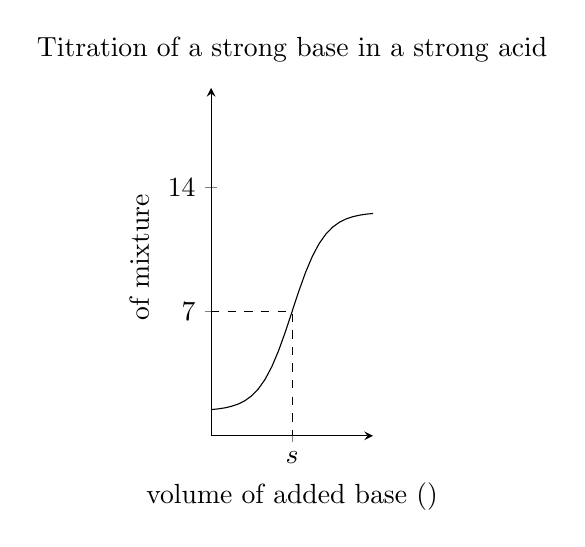
\begin{tikzpicture}
  \begin{axis}[
      width=.3\textwidth,
      height=6cm,
      title=Titration of a strong base in a strong acid,
      xlabel = volume of added base (\si{\milliliter}),
      ylabel = \pH\ of mixture,
      axis lines = left,
      xmin=0,
      %xmax=2,
      ymin=0,
      ymax=1.4,
      xtick = {2.5},
      ytick = {.5, 1},
      xticklabels = {$s$},
      yticklabels = {7, 14},
      clip = false,
    ]
    \addplot[domain=0:5]{0.8/(1 + e^(-(2*x)+5)) + 0.1};
    \draw[dashed] (0, .5) -- (2.5, .5) -- (2.5, .5) -- (2.5, 0);
  \end{axis}
\end{tikzpicture}
\hfill
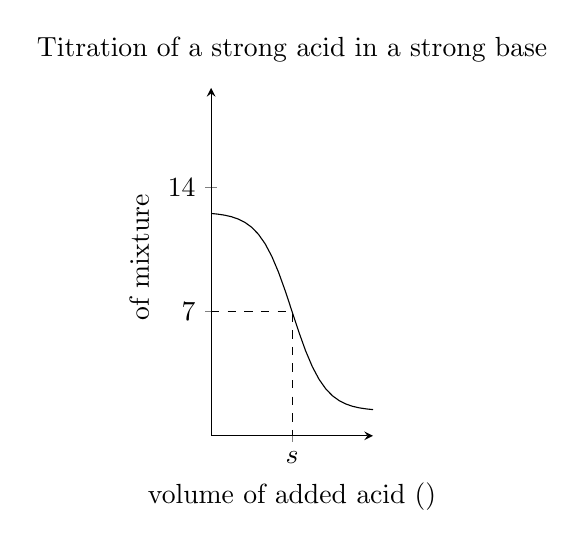
\begin{tikzpicture}
  \begin{axis}[
      width=.3\textwidth,
      height=6cm,
      title=Titration of a strong acid in a strong base,
      xlabel = volume of added acid (\si{\milliliter}),
      ylabel = \pH\ of mixture,
      axis lines = left,
      xmin=0,
      %xmax=2,
      ymin=0,
      ymax=1.4,
      xtick = {2.5},
      ytick = {.5, 1},
      xticklabels = {$s$},
      yticklabels = {7, 14},
      clip = false,
    ]
    \addplot[domain=0:5]{.9 - (.8/(1 + e^(-(2*x)+5)))};
    \draw[dashed] (0, .5) -- (2.5, .5) -- (2.5, .5) -- (2.5, 0);
  \end{axis}
\end{tikzpicture}
\hspace*{\fill}

\caption{Acid-base titration of base in an acidous solution (left) and
  acid in a basic solution (right). To the left: As we add more base
  to the solution, the \pH\ increases. The point at which the solution
  shifts from being acidic to basic, denoted $s$ in the
  diagram, is called the equivalence point, stoichiometric point and
  also the end point as it is the end volume of the titration.}
\end{hfigure}





\begin{example}[Calculating the stoichiometric point]
  We are going to calculate the (theoretical) equivalence point from
  titrating a strong base (\SI{0.250}{\molar} \ce{NaOH}) with a strong
  acid (\SI{0.340}{\molar} \ce{HCl}).

  \paragraphbreak

  This is a somewhat lengthy procedure so the steps are given i points

  \begin{enumerate}[label=\arabic*)]
  \item We begin by calculating the \pH\ of the solution before the
    equivalence point, where \SI{5.00}{\milliliter} of
    \SI{0.340}{\molar} \ce{HCl(aq)} is added to \SI{25.00}{\milliliter}
    of \SI{0.250}{\molar} \ce{NaOH(aq)}.

    \begin{enumerate}[label=\alph*)]
    \item Since \ce{NaOH} is a strong base, the amount of formed \hydroxide is
      equal to the amount of \ce{NaOH} added:
      \begin{equation*}
        \begin{split}
          \SI{0.02500}{\liter}\times\SI{0.250}{\mol\per\liter}
          =\\= \SI{6.25d-3}{\mol}~\text{of \hydroxide}
        \end{split}
      \end{equation*}

    \item We calculate the amount of \hydronium supplied by titration and
      since we add a strong acid, the amount of formed \hydronium is equal
      to the amount of added \ce{HCl}:
      \begin{equation*}
        \begin{split}
          \SI{0.00500}{\liter}\times\SI{0.340}{\mol\per\liter}
          =\\= \SI{1.70d-3}{\mol}~\text{of \hydronium}
        \end{split}
      \end{equation*}
      
    \item Find the amount (moles) of \hydroxide that remains after it
      has reacted with the added \hydronium ions.

      The stoichiometric coefficients are one-to-one so we simply subtract
      the amount of \hydronium from the amount of \hydroxide:
      \begin{equation*}
        \begin{split}
          \SI{6.25d-3}{\mol} - \SI{1.70d-3}{\mol} =\\=
          \SI{4.55d-3}{\mol}~\text{of \hydronium ions left.}
        \end{split}
      \end{equation*}
      
    \item Now we calculate the molarity of \hydroxide
      \begin{equation*}
        \frac{\SI{4.55d-3}{\mol}}{\SI{0.03000}{\liter}} =
        \SI{0.152}{\molar}
      \end{equation*}

    \item Now we can calculate the \pH\ from the hydroxide
      concentration:
      \begin{equation*}
        \pOH = - \log_{10} 0.152 = 0.818 \implies \pH = 14.00 - 0.818 = 13.18
      \end{equation*}
    \end{enumerate}

  \item Calculate the volume of \ce{HCl} needed to reach the
    equivalence point.

    We start by recognizing that, initially, there were
    \SI{6.25d-3}{\mol} of hydroxide present. Since the stoichiometric
    coefficients are one-to-one, we will have added that same amount
    of \ce{HCl} when we reach the equivalence point.

    Since we know the concentration of the acid and the number of
    moles we need, we can calculate the volume of acid:
    \begin{equation*}
      V = \frac{n}{C}
      = \frac{\SI{6.25d-3}{\mol}}{\SI{0.340}{\mol\per\liter}}
      = \SI{0.0184}{\liter}
    \end{equation*}
  \end{enumerate}
\end{example}


\begin{example}[Titration continued]
  Now, we will calculate the \pH\ of the mixture from adding extra
  \SI{1.00}{\milliliter} of hydrochloric acid after we have reached
  the equivalence point.

  \paragraphbreak

  \begin{enumerate}[label=\alph*)]
  \item Calculate the number of moles of hydronium ions formed from
    adding the additional hydrochloric acid
    \begin{equation*}
      n = \SI{0.340}{\mol\per\liter}\times\SI{1d-3}{\liter}=\SI{3.40d-4}{\mol}
    \end{equation*}

  \item If we are to calculate the concentration, molarity, of
    hydronium ions in our ``new'' mixture, we need to divide $n$ with
    the total volume, which we can sum up of

    \begin{center}
      \begin{tabular}{ll}
        the initial volume of solution & \SI{0.02500}{\liter} \\
        the titrated volume of \ce{HCl} & \SI{0.0184}{\liter} \\
        the addedvolume of \ce{HCl} & \SI{0.00100}{\liter} \\
         $\sum$ & \SI{4.44d-2}{\liter} \\
      \end{tabular}
    \end{center}

    and so
    \begin{equation*}
      [\hydronium]
      = \frac{\SI{3.40d-4}{\mol}}{\SI{4.44d-2}{\liter}}
      = \SI{7.66d-3}{\molar}
    \end{equation*}
    which makes
    \begin{equation*}
      \pH = - \log_{10} \left(\num{7.66d-3}\right) = \num{2.12}
    \end{equation*}
  \end{enumerate}
\end{example}






\subsection{Titration of weak acids and bases}



When we are titrating a weak acid with a strong base, the situation is
not as clear as it is when the species are strong acids and strong
bases. Instead the titration curve show some special characteristics,
as seen in Figure~\ref{fig:weak acid strong base}.

A weak acid will not dissociate fully, but hold on to hydrogen
atoms. This makes the \pH\ of the stochiometric point higher (more
basic) than in previous set ups.

Initially, the rise of \pH\ is steep as the strong base is added to
the acid.  The titration curve is, however, going to display a
plateau, the {\em buffering region}, where the weak acid and it's weak
base conjugate are working as a buffer and keeps the \pH\ stable in
spite of the addition of strong base. As a consequence, the titration
curve is steeper around the stochiometric point since the capacity for
forming hydronium ions have been exhausted during the passage of the
buffering region.



\begin{marginfigure}
  \begin{center}
    \begin{tikzpicture}[scale=.3]
      \draw[<->] (0, 12) -- (0, 0) -- (8, 0);
      \draw [blue] plot [smooth, tension=2] coordinates {
        (0,.4)
        (.3,1.2)
        (1,1.5)
        (3,2)
        (3.5, 7)
        (4, 9.5)
        (6, 10)
      };
    \end{tikzpicture}
  \end{center}
  \caption{The characteristics of a titration curve from titrating a
    weak acid with a strong base.\label{fig:weak acid strong base}}
\end{marginfigure}




The titration curve have three interresting points. In the middle of
the buffering region we find the {\em half-equivalence point} ($V =
V_{\text{half-eq}}$) where half of the weak acid has been converted
into it's conjugate base. Then we reach the equivalence point ($V =
V_{\text{eq}}$) of the curve where we have added the same amount of
strong base as we originally had of the weak acid, so those two
components have neutralized each other. By this point, the conjugate
base is controlling the \pH, so the \pH\ at the equivalence point will
be basic ($\pH > 7$). Beyond the equivalence point, if we add more of
the strong base, ($V > V_{\text{eq}}$) the curve develops like that
one for a strong base in water.




A titration of a strong acid into a weak base works conversely to the
weak acid/strong base previously. Initially, before we reach the
buffering region, the strong acid lowers the \pH\ rapidly, then
there's the buffering region where the buffering system of the weak
conjugates maintains the \pH. The equivalence point on the curve ($V =
V_{\text{eq}}$) reflects the fact that the weak base and the strong
acid are neutralized and the weak conjugate acid controls the \pH,
which is acidic ($\pH < 7$). As we add more strong acid, the impact of
the conjugate acid is negligible and the strong acid controls the \pH.





\begin{example}[Titration of a weak acid with a strong base]
  We will start with \SI{25.0}{\milliliter} of \SI{0.10}{\molar}
  \ce{HCOOH} ($\Ka = \num{1.77d-4}$) and add \SI{0.15}{\molar}
  \ce{NaOH}.

  \paragraphbreak

  \begin{enumerate}[label=\arabic*)]
  \item Initially $V = \SI{0}{\milliliter}$ of \ce{NaOH} is
    added. This is a weak-acid-in-water-problem. The equation for this
    reaction is
    \ceeqstar{HCOOH(aq) + H2O(l) <=> H30^+(aq) + HCOO^-(aq)}

    We set up our equilibrium table

    \begin{inlinetable}{lccccc}
        & \ce{HCOOH} & \ce{<=>} & \ce{H3O^+} & + & \ce{HCOO^-} \\
        initial & \SI{0.10}{\molar} && 0 && 0 \\
        change & $-x$ && $x$ && $x$ \\
        equilibrium & $\num{0.10} - x$ && $x$ && $x$ \\
    \end{inlinetable}
    
    And we set up the equation for equilibrium concentrations
    \begin{equation*}
      \Ka = \num{1.77d-4} = \frac{x^2}{0.10 - x}
    \end{equation*}
    which we solve for $x$. Assuming that $x \ll \text{initial
      concentration}$ will give us $x = \num{4.21d-3}$, which is
    $4.21\% < 5\%$ (assumption is okay).

    We calculate $\pH = - \log_{10}(\num{4.21d-3}) = 2.38$.

  \item We start to add strong base ($0 < V < V_{\text{eq}}$) and
    calculate the \pH\ of the mixture after we have added
    \SI{5.0}{\milliliter} of \SI{0.15}{\molar} \ce{NaOH}.

    \paragraphbreak

    Because \hydroxide is a stronger base than \ce{HCO2^-}, it reacts
    almost completely with \ce{HCOOH}.

    \ceeqstar{HCOOH(aq) + \hydroxide(aq) -> H2O(l) +
      HCO2^-(aq)\qquad K\gg 1}

    The large equilibrium constant tells us that during the reaction,
    the same number of moles of acid will dissociate as the number of
    moles ew add of the strong base, so the concentration changes from
    the titration during this part of the titration can be calculated
    using simple subtractions.

    The initial moles of formic acid is $\SI{25.0d-3}{\liter} \cdot
    \SI{0.10}{\molar} = \num{2.5d-3}$ moles. The initial moles of
    hydroxide ions is $\SI{5.0d-3}{\liter} \cdot \SI{0.15}{\molar} =
    \num{0.75d-3}$ moles.
    
    We can now calculate the number of moles after the reaction by
    subtracting the number of moles of hydroxide ions from the number
    of moles of formic acid to find the number of moles of acid that
    remains. $\num{2.5d-3} - \num{0.75d-3} = \num{1.75d-3}$ moles of
    acid. The hydroxide added will form the equal amount of the
    conjugate base, \num{0.75d-3} moles of \ce{HCO2^-}.

    Now, we have a mixture that contain {\em a weak acid and it's
      conjugate base}, which makes it a {\em buffer problem}.

    The total volume of the mixture, at this point, is
    $V = \SI{25.0d-3}{\liter} + \SI{5.0d-3}{\liter} =
    \SI{30.0d-3}{\liter}$.

    The concentrations of the conjugates are calculated by
    \begin{align*}
      \ce{[HCOOH]} = \frac{n}{V}
      &= \frac{\SI{1.75d-3}{\mol}}{\SI{30.0d-3}{\liter}}
      = \SI{5.83d-2}{\molar} \\
      \ce{[HCO2^-]} = \frac{n}{V}
      &= \frac{\SI{0.75d-3}{\mol}}{\SI{30.0d-3}{\liter}}
      = \SI{2.50d-2}{\molar} \\
    \end{align*}

    We now have two alternative ways to calculate the \pH\ at this
    point. We can either set up an equilibrium table and use the
    \Ka\ that was given earlier, or we can use the
    Henderson-Hasselbalch equation, presented earlier.

    \begin{enumerate}[label=Option \arabic*)]
    \item We set up the equilibrium table

      \begin{inlinetable}{lccc}
          & \ce{HCOOH} & \ce{H3O^+} & \ce{HCO2^-} \\
          initial M & \num{5.83d-2} & 0 & \num{2.50d-2} \\
          $\Delta\si{\molar}$ & $-x$ & $x$ & $-x$ \\
          at equilibrium & $\num{5.83d-2} - x$ & $x$ & $\num{2.50d-2} + x$ \\
      \end{inlinetable}

      We plug this into an equation
      \begin{equation*}
        \Ka = \num{1.77d-4} = \frac{x(\num{2.50d-2} + x)}{\num{5.83d-2} - x}
      \end{equation*}

      We now make the assumption that $x$, the percentage protonized,
      turns out to be ``small enough'' (less than five percent of any
      of the initial concentrations) to be negligible as a term on
      it's own in the equation. This enable us to simplify the
      equation to
      \begin{equation*}
        \num{1.77d-4} = \frac{\num{2.50d-2}x}{\num{5.83d-2}}
      \end{equation*}
      which we solve for $x$ and turns out to $x = \num{4.13d-4}$,
      fortunately less than five percent of both initial
      concentrations (1.65\% and 0.7\%, respectively) so our
      assumption stands.

      Now, $\pH = -\log_{10}(\num{4.13d-4}) = 3.38$ as we have added
      $V = \SI{5.0}{\milliliter}$ of \ce{NaOH}.

    \item Using the Henderson-Hasselbalch equation, we calculate
      \ceeqstar{\pH \approx \pKa - \log_{10}\frac{[HA]}{[A^-]}}

      If we plug our values into the equation we get
      \begin{equation*}
        \pH \approx 3.75 - \log_{10}\frac{\num{5.83d-2}}{\num{2.50d-2}}
        = 3.75 - 0.368 = 3.38
      \end{equation*}

      Checking assumption (for the equation) we see that the change in
      concentrations (given here as $\ce{[H3O^+]}$), $\ce{[H3O^+] =
        \num{4.2d-4}}$ is clearly less than five percent of the
      initial concentrations.

      Again $\pH = 3.38$ as with the other option.
    \end{enumerate}

  \item At the {\em half-equivalence point}, the volume of \ce{NaOH}
    added is the half of the amount of the equivalence volume. This is
    the ``middle'' of the buffering region so \ce{[HA] = [A^-]} and
    \begin{equation*}
      \pH \approx \pKa - \log_{10}\frac{\ce{[HA]}}{\ce{[A^-]}}
      = \pKa = 3.75
    \end{equation*}

  \item At {\em the equivalence point} ($V = V_{\text{eq}}$), the
    amount of sodium hydroxide equals the original amount of formic
    acid. The \pH\ depends on the {\em salt} formed. Our principles to
    decide this (see Section~\ref{sec:salt problems}) let us conclude
    that since formic acid and sodium hydroxide form \ce{NaHCO2} and
    water. The sodium ion is neutral with respect to \pH\ but
    \ce{HCO2^-} is a base so the aqueous solution of \ce{NaHCO2} will
    be basic.

    At this point, all of the formic acid is converted into it's
    conjugate base.

    We calculate the \pH\ at the equivalence point.
    \begin{enumerate}[label=\roman*)]
    \item We start by using the known value of the number of moles of
      \ce{CHOOC} from before, which is \num{2.5d-3} moles. This amount
      equals the amount of \ce{HCO2^-} formed as well as the amount of
      \hydroxide added.

      The volume of solution of \ce{NaOH} is given by
      \begin{equation*}
        V_{\ce{NaOH}} = \frac{n}{C}
        = \frac{\SI{2.5d-3}{\mol}}{\SI{0.15}{\mol\per\liter}}
        = \SI{1.67d-2}{\liter}
      \end{equation*}

      So the total volume is the sum of volumes added:
      $\num{25d-3} + \num{1.67d-2} \si{\liter}=
      \SI{4.17d-2}{\liter}$.

    \item By calculating the molarity of the conjugate base we find
      out the concentration of hydroxide ions
      \begin{equation*}
        [\hydroxide]
        = \frac{\SI{2.5d-3}{\mole}}{\SI{4.17d-2}{\liter}}
        = \SI{6.00d-2}{\molar}
      \end{equation*}

      We set up an equilibrium table for the equilibrium
      \ceeqstar{HCO2^-(aq) + H2O(l) <=> HCOOH(aq) + OH^-(aq)}

      \begin{inlinetable}{lccc}
        & \ce{HCO2^-} & \ce{HCOOH} & \ce{OH^-} \\
        initial M & 0.0600 & 0 & 0 \\
        change & $-x$ & $x$ & $x$ \\
        at equilibrium & $0.0600 - x$ & $x$ & $x$ \\
      \end{inlinetable}

      Now, solving
      \begin{equation*}
        \Kb = \num{5.6d-11} = \frac{x^2}{0.0600 - x}
      \end{equation*}
      for $x$ ($\Kb = \num{5.6d-11}$ for \ce{HCO2^-} in water),
      assuming $x$ is negligible ($x \ll 0.0600$) allow us to
      calculate $x$ (which is equal to $[\hydroxide]$) as
      \begin{align*}
        x^2 &= \num{5.6d-11} \cdot 0.0600 \\
        x &= \num{1.83d-6}
      \end{align*}
      
      This give us $\pOH = -\log_{10}[\hydroxide] =
      -log_{10}(\num{1.83d-6}) = 5.74$ and this give us $\pH = 14.00 -
      \pOH = 8.26$ which is basic.
    \end{enumerate}
  \item Beyond the equivalence point ($V > V_{\text{eq}}$) we continue
    to add sodium hydroxide to the solution of formate (\ce{CHO2^-},
    IUPAC name: methanoate). At this point, the formate does not add
    much hydroxide ions beyond the \SI{1.83d-6}{\molar} at the
    equivalence point so \pH\ and \pOH\ will be controlled by the
    amount of sodium hydroxide added. This is now similar to a strong
    acid in water problem or a strong base in water problem.

    \paragraphbreak

    At \SI{5.00}{\milliliter} past the equivalence point, we have
    \begin{equation*}
      n = \SI{5.00d-3}{\liter} \cdot \SI{0.15}{\mol\per\liter}
      = \SI{7.5d-4}{\mol}
    \end{equation*}
    of excess hydroxide ions.

    By now, our total volume of solutions is $V = \num{5d-3} +
    \num{2.5d-2} + \num{1.67d-2} = \SI{4.67d-2}{\liter}$. Now
    \begin{equation*}
      [\hydroxide] = \frac{n}{V}
      = \frac{\SI{7.5d-4}{\mol}}{\SI{4.67d-2}{\liter}}
      = \SI{1.61d-2}{\molar}
    \end{equation*}
    and $\pOH = -\log_{10}(\num{1.61d-2}) = 1.79$ from which we can
    calculate $\pH = 14.00 - \pOH = 12.21$, which is basic.

    We also see that the concentration of hydroxide ions from the
    conjugate base at the equilibrium point (\num{1.83d-6}) is far too
    small to be of any significance, which we assumed earlier.
  \end{enumerate}

  A plot of the found values on the titration curve is seen below.
  
  \begin{center}
    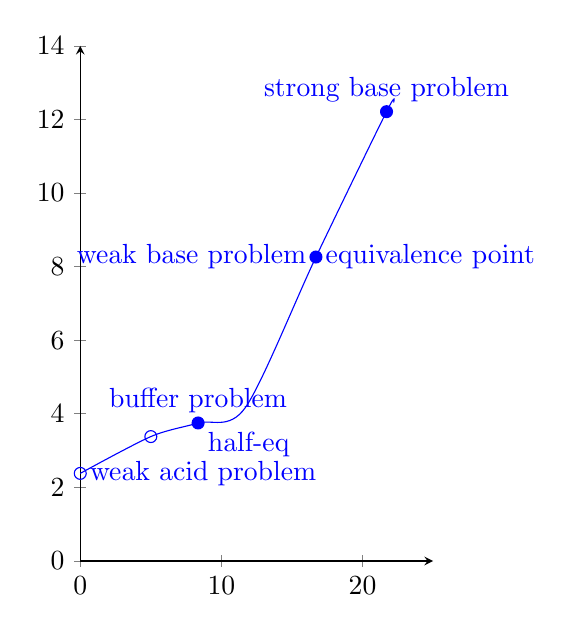
\begin{tikzpicture}
      \tikzstyle{marker} = [blue]
      \begin{axis}[
          width=.5\textwidth,
          height=.67\textwidth,
          axis lines=left,
          xmin=0,
          xmax=25,
          ymin=0,
          ymax=14,
          clip=false
        ]
        \addplot[blue, smooth] coordinates {
          (0, 2.38)     % initial
          (5, 3.38)     % 5ml in
          (8.35, 3.75)  % half-eq
          (11.7, 4.17)
          (16.7, 8.26)  % eq
          (21.7, 12.21)
          (22.2, 12.46)};
        \draw[marker] (0, 2.38) circle (.5ex)
        node[anchor=west]{weak acid problem};
        \draw[marker] (5, 3.38) circle (.5ex);     % 5ml in
        \draw[marker, fill=blue] (8.35, 3.75) circle (.5ex)
        node[above]{buffer problem}
        node[anchor=north west]{half-eq};
        \draw[marker, fill=blue] (16.7, 8.26) circle (.5ex)
        node[left]{weak base problem}
        node[right]{equivalence point};
        \draw[marker, fill=blue] (21.7, 12.21)  circle (.5ex)
        node[above]{strong base problem};
      \end{axis}
    \end{tikzpicture}
  \end{center}

\end{example}



\end{document}
